Este capítulo é onde começamos a abordar nosso modelo proposto de um sistema de arquivos distribuídos tolerante a falhas. Iniciamos com um visão geral da arquitetura do sistema apresentando detalhes do serviço de metadados, serviço de armazenamento,, servidor e do cliente. Em seguida é abordado as operações realizadas pelo sistema de arquivos distribuído proposto, tais operações estão divididas entre operações do tipo Cliente-Servidor e Servidor-Servidor. Seguindo com o capítulo, é explanado como foi realizada a implementação do sistema de arquivos distribuído utilizando conceitos de RAID proposto, focando especialmente nos serviços de metadados e de armazenamento, além dos clientes. Enfim, o capítulo finaliza apresentado o planejamento e execução dos experimentos seguido da análise dos dados obtidos.


	\section{Arquitetura do sistema}
	
	A arquitetura do Sistema de Arquivos Distribuídos proposto neste trabalho é composto por um ou vários clientes comunicando-se com ao menos três servidores de metadados e quatro servidores de armazenamento, onde cada um deles está conectado através de Internet ou outra rede, como a Figura~\ref{fig:vis_sis}  sintetiza. Neste sistema, cada servidor de armazenamento se comporta como um disco rígido em sistema de RAID, armazenando distribuidamente as partes dos arquivos e/ou paridades associadas. \\
	
	
	%O nosso objeivo neste artigo é a construção de um SAD baseado na computação em nuvem que possui menor \textit{overhead} de espaço, comparado a 200\% de método de replicação, sem degradar muito o performance e segurança de dados. 
	%Para isso, nós observamos em técnica de redundância usado na tecnologia RAID, onde consegue diminuir o espaço ocupado pela parte redundante com atribuição de paridade nos arquivos, ao invés de simples replicação. Na mesma tecnologia também foi 

	
	
	\begin{figure}[htb]
		\begin{center}
			
			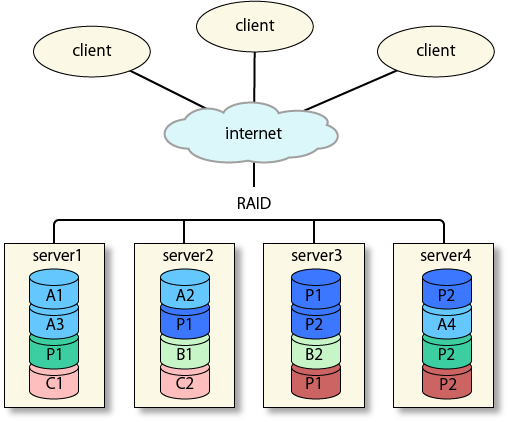
\includegraphics[clip,width=10.0cm]{images/image1.png}
			\caption{Visão geral do sistema}
			\label{fig:vis_sis}
		\end{center}
	\end{figure}
	
	Em um sistema de arquivos local, normalmente o metadado e o conteúdo de um arquivo são armazenados na mesma unidade de armazenamento. No caso de um SAD, como um arquivo pode ser armazenados distribuidamente entre servidores diferentes, os metadados são espalhados por vários servidores, tendo assim, a necessidade de fazer a busca para acessar em um determinado metadado. Obviamente essa busca consome recursos operacionais, relativamente alta por tratar de uma transmissão na rede.   \\
	
	\begin{figure}[htb]
		\begin{center}
			
			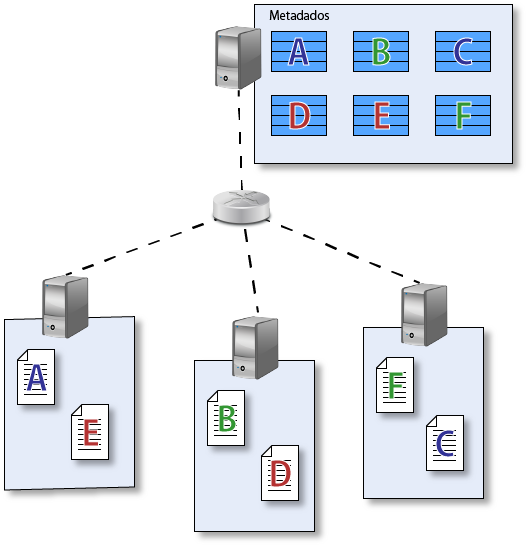
\includegraphics[clip,width=10.0cm]{images/image7.png}
			\caption{\textit{Name node} e \textit{data node}}
			\label{fig:namenode}
		\end{center}
	\end{figure}
	
	\subsection{Serviço de Metadados}
		Grupo de servidores que fazem o gerenciamento dos dados.\\
		
		Em nosso sistema utilizamos o conceito de blocos, onde um bloco é um conjunto de dados de um dado arquivo ou os dados de paridade de um determinado arquivo. O tamanho do bloco é determinado levando em consideração a quantidade de servidores de armazenamento ativos, ou seja, se houverem quatro servidores ativo, então o arquivo (independente de seu tamanho) será dividido em quatro blocos de tamanhos idênticos, caso seja necessário, o ultimo bloco será preenchido com bits '0' até que o bloco alcance o tamanho previamente fixado.
		\\ 
		
		O Serviço de metadados, também conhecido por \textit{name node}, é o conjunto de servidores que gerencia as informações dos arquivos armazenados, utilizando-se dos metadados. Em nosso sistema a data de criação, data da ultima modificação, data do ultimo acesso, tamanho, identificador do bloco de dados e nome do servidor são considerados metadados. 
		\\
		
		É da responsabilidade do sistema de metadados gerenciar a comunicação entre cliente e servidores de armazenamento (ou  \textit{data nodes}), utilizando-se das informações que indicam  estado atual do sistema e qual o tipo de RAID está sendo utilizado (apenas um tipo de RAID pode ser utilizado por operação) o \textit{name node} deve decidir em quantos blocos de tamanho idêntico o arquivo deve ser dividido e em quais servidores de armazenamento cada bloco deve ser armazenado.
		\\ 
		
		Nosso sistema está preparado para tratar os seguintes tipos de RAID, os quais foram explorados com maior profundidade no capítulo 4.
		\\
		
		\begin{itemize}
			\item RAID 0 - fracionamento simples;
			\item RAID 1 - espelhamento;
			\item RAID 5 - fracionamento com paridade espalhada entre os discos do vetor.
		\end{itemize}
		
		O Serviço de metadados mantém na sua memória local a árvore de diretórios, o que indica localização lógica dos arquivos. Quando recebe uma solicitação de cliente por um arquivo, pesquisa a sua árvore de diretórios para identificar qual diretório que este arquivo se encontra. Como resultado da pesquisa obtém o metadado do arquivo referente, conseguindo descobrir a sua localização física, a lista dos todos os \textit{data nodes} que possuem as partes do arquivo.
		\\
		
		Por sua propriedade como um interface entre clientes e \textit{data nodes}, a ocorrência de alguma falha na operação ou indisponibilidade causada pela queda do servidor tem  enorme influencia na execução do sistema, podendo até resultar em parada total do sistema. Assim, é muito importante elaborar uma esquema para manter o \textit{name node} protegidos contra falhas ou queda total. Em nosso sistema usaremos a biblioteca BFT-SMaRt, que fornece tolerância a falha no serviço através de replicação por máquina de estado. \\
	
	\subsection{Serviço de Armazenamento}
		Grupo de servidores responsáveis pelo armazenamento físico dos dados gerenciados pelo sistema de metadados. Também conhecido como \textit{data nodes}.\\
		
		Em nosso sistema, o serviço de armazenamento não possui a necessidade de saber qual tipo de RAID está sendo executado, a responsabilidade de manter o RAID consistente é toda do serviço de metadados. Desta forma, o sistema de armazenamento apenas se conecta a uma porta e fica aguardando algum cliente se conectar a sua respectiva porta. Quando algum cliente conecta-se na porta do servidor, é realizado um \textit{handshake} preliminar, logo em seguida o cliente inicia a transferência dos dados que devem ser guardados pelo sistema de armazenamento. Ao fim da transferência o cliente fecha a conexão, enquanto o sistema de armazenamento indexa o arquivo recebido utilizando as informações adicionais que o serviço de metadados anexou ao arquivo. Com tais informações é possível saber o identificador tanto do arquivo quanto do cliente que o enviou. Tais dados adicionais são necessários para garantir que apenas o usuário dono dos dados enviados tenha acesso a eles, além de possibilitar identificar quais dados o cliente deseja receber de forma simples e eficiente.  
		\\
	
	\subsection{Cliente}
	O programa cliente executado no computador do usuário final de nosso sistema. 
	\\
	
	Para cada operação que deseje realizar, o programa cliente (doravante Cliente) deve primeiramente comunicar-se com o serviço de metadados, o qual ou irá realizar a operação (no caso de operações envolvendo diretórios) ou informar com quais servidores de armazenamento o cliente deve se comunicar e quais blocos devem ser enviados para cada servidor (no caso de operações envolvendo arquivos). Entretanto, é função do Cliente informar qual tipo de RAID ele deseja utilizar.
	\\
	
	Após a comunicação inicial com o serviço de metadados, caso o cliente solicite pelo \textit{upload} ele deve iniciar a comunicação com os servidores de dados informados pelo serviço de metadado. Caso o cliente tenha decidido utilizar o RAID 5, é ele quem fica responsável por calcular a paridade do arquivo, isto deve-se ao fato de que apenas o cliente conhece o arquivo. O procedimento para o calculo da paridade é exemplificado na figura~\ref{fig:img6}. Outra atribuição do cliente é a partição do arquivo em blocos de iguais tamanhos, cada bloco será enviado para um dos servidores de dados informado pelo metadado, ou seja, o arquivo deve ser fragmentado de tal forma que cada servidor receba um bloco de dados, frisando que no caso do RAID 5 um dos blocos deve conter apenas informações de paridade previamente calculado pelo cliente. 
	\\
	
		\begin{figure}[htb]
			\begin{center}
				
				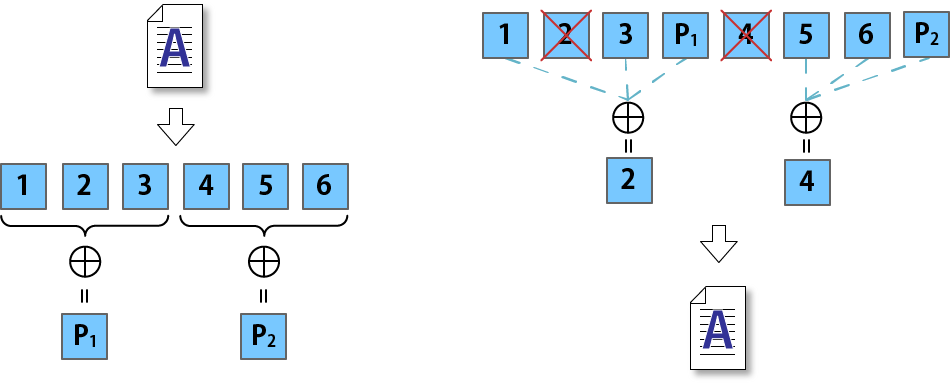
\includegraphics[clip,width=15.0cm]{images/image6.png}
				\caption{Geração de paridade}
				\label{fig:img6}
			\end{center}
		\end{figure}
	
	Caso a operação desejada pelo usuário final seja a de \textit{download} de algum de seus arquivos, o cliente deve coletar as informações de quais servidores possuem os blocos do arquivo almejado e quais as informações de identificação de cada bloco através do servidor de metadado. Com posse de tais informações, o cliente deve iniciar a comunicação com cada um dos servidores de dados apresentando a identificação de qual bloco cada servidor de dados deve enviar. Quando todos os servidores acabarem seus envios, o cliente deve usar os dados em sua posse para unir todos os blocos e recriar o arquivo desejado pelo usuário. Obviamente, esta descrição genérica da operação vai sofrer leves alterações dependendo de qual opção de RAID o cliente esteja utilizando. Para a opção de RAID 5, é possível que um dos blocos recebidos pelo cliente seja um bloco de paridade, para esse caso, o cliente deve utilizar as informações dos outros blocos para determinar qual é o bloco de dados faltante e utilizar a paridade para recuperar tal bloco. A Figura~\ref{fig:img2} mostra um esquema simplificado da operação de recuperar um arquivo realizado pelo lado do cliente.
	\\
	
	\begin{figure}[htb]
		\begin{center}
			
			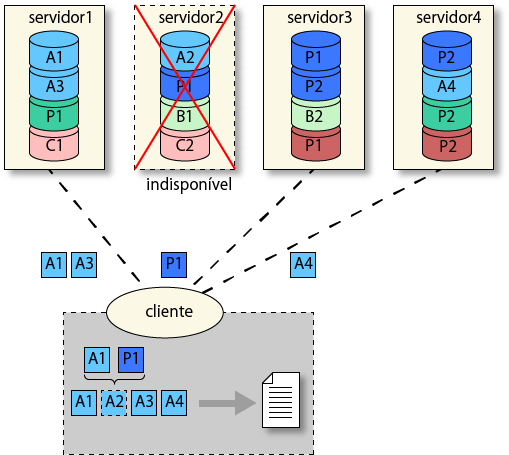
\includegraphics[clip,width=10.0cm]{images/image2.png}
			\caption{Recuperando um arquivo de uma falha}
			\label{fig:img2}
		\end{center}
	\end{figure}
	
	\section{Operações no Sistema de Arquivos Distribuídos}
	
	Nesta seção serão apresentadas as operações básicas que o nosso SAD executa. Tais operações podem ser divididas em dois grupos dependendo das entidades envolvidas. O primeiro deles é entre cliente e servidor, composta por operações envolvendo solicitações de ações do cliente para o servidor. O segundo tipo é as operações que ocorrem entre servidores, voltadas para o gerenciamento do serviço sendo que este tipo de operações deve ocorrer de forma transparente para o cliente.
	\\
	
	\subsection{Cliente-Servidor}
	
	É um conjunto de operações semelhantes a que são implementadas em um sistema de arquivos local, aquele que é integrado na maioria dos sistemas operacionais comuns. Composto pelas operações sobre arquivos e pastas e suas execuções podem ocorrer entre cliente e \textit{name node} ou cliente e \textit{data node}.
	
	\subsubsection{Criar arquivo}
	
	Operação realizada inicialmente entre o cliente e o servidor do tipo \textit{name node}. Nesse primeiro momento o cliente informa ao \textit{name node} que deseja criar um novo arquivo e em qual diretório ele deve ser criado, além de enviar os metadados do arquivo que pretende enviar. Com posse dessas informações e de qual RAID o cliente está operando, o servidor de metadados processa e transmite para o cliente para quais \textit{data node} os blocos do arquivo devem ser enviados e qual a identificação de cada bloco. O processamento de tais informações é diretamente influenciado pelo estado atual do sistema, o \textit{name node} leva em consideração a disponibilidade de cada \textit{data node} e o quanto de espaço livre em disco cada um possui.
	\\
	
	A segunda parte da operação é realizada entre o cliente e os servidores do tipo \textit{data node}. Após a comunicação com o servidor de metadados, o cliente sabe para quantos \textit{data nodes} o seu arquivo será enviado, desta forma, o cliente fragmenta o arquivo de forma que cada \textit{data nodes} irá receber um bloco de tamanho uniforme. Caso o sistema esteja usando o RAID 5, o cliente ainda deve calcular o bloco de paridade do arquivo e enviar para um dos \textit{data nodes}.
	\\
	
	\subsubsection{Criar diretório}
	
	Operação realizada exclusivamente entre o cliente e o servidor \textit{name node}. Nessa operação o cliente informa ao \textit{name node} que deseja criar um diretório, passando como metadados apenas o nome do novo diretório e o nome de seu diretório pai. Com tais informações, o servidor de metadados primeiramente verifica se já existe um diretório com o mesmo nome no diretório pai, em caso negativo ele atualiza a arvore de diretório do cliente. No caso de já existir um diretório com mesmo nome, o cliente é informado e o novo diretório não é criado.
	\\
	
	\subsubsection{Abrir arquivos}
	
	Operação realizada inicialmente entre o cliente e o servidor do tipo \textit{name node}. Nesse primeiro momento o cliente informa ao \textit{name node} que deseja abrir um arquivo, para tal, o cliente deve fornecer o nome do arquivo e o nome do diretório onde ele está. A primeira ação do servidor de metadados é verificar se o arquivo de fato existe no diretório informado, em caso positivo ele deve verificar se o cliente possui acesso ao arquivo. No caso do cliente possuir acesso, o \textit{name node} verifica em quantos blocos o arquivo foi dividido e em quais \textit{data nodes} cada bloco foi armazenado, após coletar tais informações, o servidor de metadados informa ao cliente quais servidores de dados ele, o cliente, deve se comunicar e o identificador de cada bloco. Para o caso de o arquivo não existir no diretório informado ou do cliente não possuir acesso para tal arquivo, o servidor de metadados deve envia ruma mensagem de erro informando a indisponibilidade do arquivo solicitado. 
	\\
	
	A segunda parte da operação é realizada entre o cliente e os servidores do tipo \textit{data node}. Após a comunicação com o servidor de metadados, o cliente sabe em quais \textit{data nodes} os blocos de seu arquivo estão armazenados. Desta forma, o cliente inicia a comunicação com cada \textit{data node} informado. A comunicação procede da seguinte forma, o cliente informa o identificador do bloco que deseja receber, enquanto que o \textit{data node} apenas verifica a existência do bloco informado. Em caso positivo, o bloco é enviado para o solicitante e em caso negativo, uma mensagem de erro alertando sobre a inexistência do bloco informado. Repare que o \textit{data node} não realiza nenhuma operação de controle de acesso sobre o bloco.
	\\
	
	A terceira parte da operação é realizada exclusivamente pelo cliente. Nesta ultima parte, o cliente é responsável por unir todos os blocos recebidos e recriar o arquivo almejado.  Vale ressaltar que essa operação sofre variações dependo do RAID sendo utilizado. Para o caso do RAID 5, um dos blocos recebido pelo cliente pode ser um bloco de paridade, nesse caso, antes de recriar o arquivo o cliente deve utilizar as informações de paridade contidas em tal bloco para recuperar o bloco faltante.
	\\
	
	\subsubsection{Abrir diretório}
	 
	 Operação realizada exclusivamente entre o cliente e o servidor \textit{name node}. Nessa operação o cliente informa ao \textit{name node} que deseja abrir um diretório, passando como metadados apenas o nome do novo diretório almejado e do diretório atual. A primeira ação do servidor de metadados é verificar a existência do diretório solicitado, em caso positivo, o servidor também checa se o cliente possui permissão de acesso e se o diretório está livre. Caso todas as validações sejam positivas, o servidor muda o diretório atual do cliente para o diretório solicitado. Caso algum problema seja detectado, uma mensagem de erro é disparada para o cliente e o seu diretório atual não é alterado.
	 \\
	 %PAREI AQUI!!!!!!!!!!!!!!!!!!!!!!!!!!!!!!!!!!!!!!!!!!!!!!!!!!!!!!!!!!!!!!!!!!!!!!!!!!!!!!!%
	 
	\subsubsection{Deletar arquivos}
	Deletar um arquivo vai seguir procedimentos semelhantes a operação de abrir arquivo. Em primeiro lugar recebe o nome e diretório do arquivo a ser apagado. Faz a busca pela árvore de diretórios para achar o diretório requisitado, e chegando em diretório correto, procura o arquivo por nome. Quando encontra o arquivo desejado, verifica se está satisfazendo as condições para efetuar a operação, checando a permissão de acesso e estado de bloqueio do arquivo.  
	
	\subsubsection{Fechar um arquivo aberto}
	
	Fechar o arquivo aberto por um cliente.
	
	\subsubsection{Editar um arquivo}
	
	Fazer alteração no arquivo armazenado.
	
	\subsubsection{Modificar metadado}
	
	Permite fazer alterações sobre as informações do arquivo, editando diretamente o metadado associado.
	
	
	\subsection{Servidor-Servidor}
	São operações ocorridos entre \textit{name node} e \textit{data node}, com função de gerenciamento de SAD.
	
	\subsubsection{Receber arquivo criado}
	
	Na operação de criar arquivo, o \textit{name node} define quais \textit{data nodes} vão ser utilizados para armazenar os fragmentos de arquivo a ser criado, calculando a melhor forma para distribuir igualmente a carga entre os \textit{data nodes}. Dessa forma, além de informar o cliente quais são os servidores que deve enviar os dados, deve avisar os \textit{data nodes} que vai chegar dados enviados pelo cliente.
	
	\subsubsection{Apagar arquivo deletado}
	
	Deleta os dados pertencentes ao arquivo solicitado para exclusão.
	
	\subsubsection{Transferir dados entre servidores}
	
	Transferência de arquivos entre \textit{data nodes}.
	
	
	\section{Implementação}
	
	\subsection{Serviço de Metadados}
	
	\subsection{Serviço de Armazenamento}
	
	\subsection{Cliente}
	
	
	
	